\documentclass{article}
\usepackage[a4paper, margin=1in]{geometry}
\usepackage[T1]{fontenc}
\usepackage[utf8]{inputenc}
\usepackage{amsmath, amssymb, graphicx, hyperref}
\usepackage{bookmark}
\graphicspath{{../figures/}}
\usepackage[framed,numbered]{matlab-prettifier}
\usepackage{xcolor}
\usepackage{listings}

\geometry{a4paper, margin=1in}

% MATLAB code style
\lstset{
  style      = Matlab-editor,
  basicstyle = \mlttfamily,
  breaklines = true
}

\title{\textbf{Practical - 8}}
\author{}
\date{October 24, 2026}

\pagenumbering{gobble}

\begin{document}
\maketitle

\noindent
\textbf{\large{Aim:}} To model the effect of a single cold pill and a course of cold pills.

\vspace{1em}
\noindent
\textbf{\large{Theory:}}

\begin{center}
    \textbf{\underline{SINGLE COLD PILL}}
\end{center}

\noindent
\underline{Idea:} Suppose a person takes one cold pill. After the pill is absorbed, the medicine in the body gradually decreases because the body removes/eliminates the drug.

\noindent
\underline{Assumption:} The rate at which the drug leaves the body is proportional to the amount of drug currently present.

\noindent
Therefore,
\[\frac{dP}{dt} = - kP\]
\begin{itemize}
    \item $P(t) =$ amount of medicine at time $t$
    \item $t =$ time
    \item $k =$ elimination rate constant
    \item $P0 =$ initial amount
\end{itemize}
The negative sign indicates that the amount of medicine decreases with time.

\noindent
Example:

Take $P0 = 100$ mg and $k = 0.2$. Thus,
\[\frac{dP}{dt} = -0.2P, \quad P(0) = 100\]
\underline{Solution:} Separating variables and integrating gives $P(t) = 100e^{-0.2t}$, using $P(0) = 100$ gives:
\begin{center}$P(t) = 100e^{-0.2t}$ (exponentially decay curve)\end{center}

\vspace{2em}
\begin{center}
    \textbf{\underline{COURSE OF COLD PILLS}}
\end{center}

\noindent
Repeated Doses

\noindent
In a course of pills, a new dose is taken after a fixed time interval. The medicine already present continues to decay, while the new pill adds a fixed amount.

\noindent
Example: dose = 100 mg every 6 hours. The doses occur at $t =$ 0, 6, 12, 18 and 24 hours.

\noindent
Between two doses, medicine still follows,
\[\frac{dP}{dt} = -kP\]
but whenever a new pill is taken, 100 mg is added suddenly. This produces a graph that repeatedly falls and jumps upward. 

\vspace{1em}
\noindent
\textbf{What different happens here?}

\noindent
For one pill,
\[P(t) = 100e^{-0.2t}\]
For a course of pills, we have several doses. 

\vspace{0.5em} \noindent
The first pill contributes:
\[100e^{-0.2t}\]
The second pill is taken at $t = 6$, so the contribution after $t = 6$ is:
\[100e^{-0.2(t-6)}\]
The third pill contributes:
\[100e^{-0.2(t-12)}\]
And so on.

\vspace{1em}
\noindent
Therefore, after the third dose, for example:
\[P(t) = 100e^{-0.2t} + 100e^{-0.2(t-6)} + 100e^{-0.2(t-12)}\]
This is the superposition of the remaining amounts from each dose.

\vspace{1em}
\noindent
What is Heaviside function? It acts like a \textbf{switch}. 

\vspace{0.5em}
\noindent
For Example:
\[H(t-6)\]
is approximately
\[H(t-6) = \begin{cases} 0, & t < 6 \\ 1, & t \geq 6 \end{cases}\]
So, the second pill's contribution
\[100e^{-0.2(t-6)}\]
doesn't begin until
\[t = 6\]
Similarly, heaviside(t) $\rightarrow$ first pill $\rightarrow$ heaviside($t-6$) $\rightarrow$ second pill $\rightarrow$ heaviside($t-12$) $\rightarrow$ third pill $\rightarrow$ heaviside($t-18$) $\rightarrow$ fourth pill $\rightarrow$ heaviside($t - 24$)

\vspace{1em}
\noindent
\textbf{Parameters:}

\noindent
Dose, $D = 100$ mg

\noindent
Elimination constant, $k = 0.2$

\noindent
Time interval between pills, $\Delta t = 6$ hours

\noindent
Number of pills, $N = 5$

\vspace{1em}
\noindent
\textbf{\large{MATLAB Code (Single Cold Pill):}}

\begin{lstlisting}
clc; clear all; close all;

syms P(t)

k1 = 0.1;
k2 = 0.2;
k3 = 0.5;
P0 = 100;

% For k1

eqn1 = diff(P,t) == -k1*P;

init1 = P(0) == P0;

PSol1 = dsolve(eqn1,init1);

disp(PSol1);

% For k2

eqn2 = diff(P,t) == -k2*P;

init2 = P(0) == P0;

PSol2 = dsolve(eqn2,init2);

disp(PSol2);

% For k3

eqn3 = diff(P,t) == -k3*P;

init3 = P(0) == P0;

PSol3 = dsolve(eqn3,init3);

disp(PSol3);

% Graph Plotting
fplot(PSol1, [0 20], 'LineWidth',2, Color='r');
hold on
fplot(PSol2, [0 20], 'LineWidth',2, Color='b');
hold on
fplot(PSol3, [0 20], 'LineWidth',2, Color='g');
grid on
xlabel('Time')
ylabel('Amount of Medicine (mg)')
title('Single Cold Pill')
legend('Elemination 1', 'Elimination 2', 'Elimination 3')
\end{lstlisting}

\vspace{1em}
\noindent
\textbf{\large{Output (Single Cold Pill):}}
\begin{flushleft}
    $100\,{\mathrm{e}}^{-\frac{t}{10}}$
\end{flushleft}
\begin{flushleft}
    $100\,{\mathrm{e}}^{-\frac{t}{5}}$
\end{flushleft}
\begin{flushleft}
    $100\,{\mathrm{e}}^{-\frac{t}{2}}$
\end{flushleft}
\begin{figure}[htbp]
    \centering
    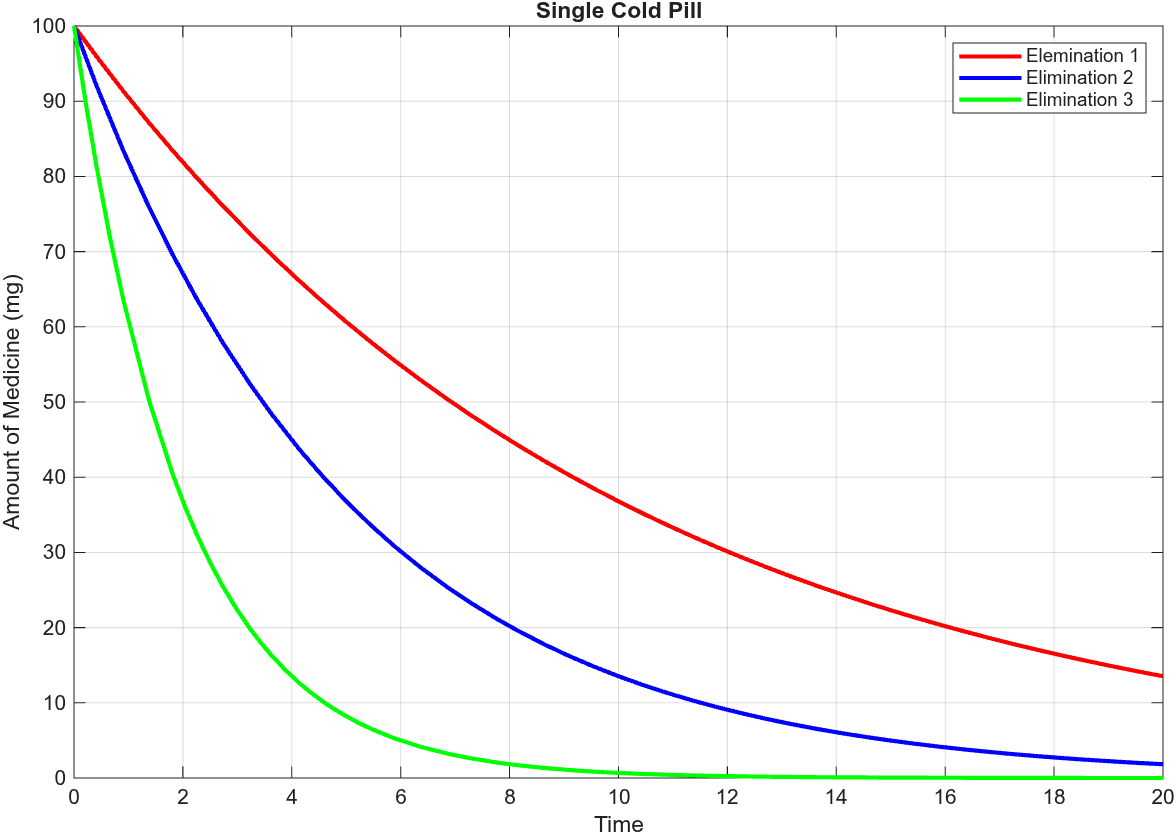
\includegraphics[width=0.7\textwidth]{Figure8.1.png}
\end{figure}

\newpage
\noindent
\textbf{\large{MATLAB Code (Course of Cold Pills):}}
\begin{lstlisting}
clc; clear all; close all;

syms P(t)

% Parameters
D = 100;
k = 0.2;
tau = 6;
N = 5;

% Differential Equation for elimination 
eqn = diff(P,t) == -k*P;

% Initial condition for one dose
init = P(0) ==D;

% Solve using dsolve
PSol = dsolve(eqn,init);

disp('Solution after one dose:')
disp(PSol)

% Total amount of repeated doses
Ptotal = 0;

for n = 0:N-1
    Ptotal = Ptotal + D*exp(-k*(t-n*tau))*heaviside(t-n*tau);
end

% Plot
fplot(Ptotal, [0 N*tau], 'LineWidth',2)

grid on
xlabel('Time (hours)')
ylabel('Amount of medicine (mg)')
title('Course of Cold Pills')
\end{lstlisting}

\vspace{1em}
\noindent
\textbf{\large{Output (Course of Cold Pills):}}
\begin{flushleft}
\tiny{Solution after one dose:}
\end{flushleft}
\begin{flushleft}
    $100\,{\mathrm{e}}^{-\frac{t}{5}}$
\end{flushleft}
\begin{figure}[htbp]
    \centering
    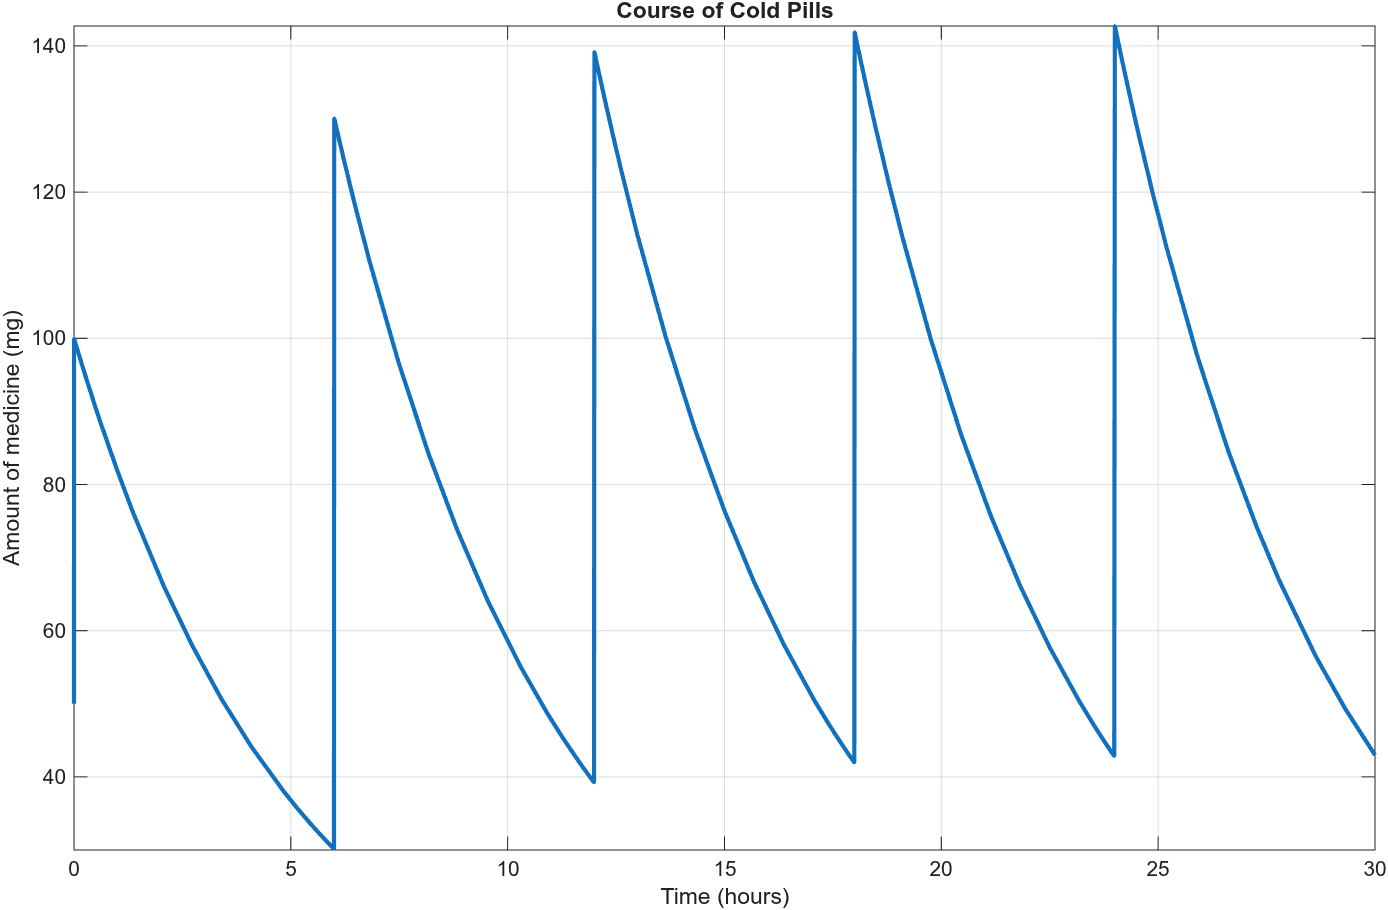
\includegraphics[width=0.7\textwidth]{Figure8.2.png}
\end{figure}

\vspace{1em}
\noindent
\textbf{\large{Observation:}} 

\vspace{0.5em}
\noindent
\large{SINGLE COLD PILL:}

\noindent
The amount of medicine decreases rapidly at first and then more slowly.

\noindent
Effect of $k$: Take $k = 0.1, 0.2, 0.5$

\noindent
smaller $k \rightarrow$ slower elimination $\rightarrow$ medicine remains longer

\noindent
larger $k \rightarrow$ faster elimination $\rightarrow$ medicine leaves more quickly

\noindent
This is an exponential decay model. The negative sign represents elimination. Increasing k makes the decay faster.

\vspace{1.5em}
\noindent
\large{COURSE OF COLD PILLS:}

\noindent
After each pill, the amount of medicine increases suddenly. Between two pills, the amount decreases exponentially because the medicine is being eliminated.

\end{document}
